\documentclass[UTF8]{article}


% if you need to pass options to natbib,use,e.g.:
%     \PassOptionsToPackage{numbers,compress}{natbib}
% before loading neurips_2022


% ready for submission
\usepackage[final]{neurips_2022_zh}

% \PassOptionsToPackage{numbers,compress}{natbib}


% to compile a preprint version,e.g.,for submission to arXiv,add add the
% [preprint] option:
%     \usepackage[preprint]{neurips_2022}


% to compile a camera-ready version,add the [final] option,e.g.:
%     \usepackage[final]{neurips_2022}


% to avoid loading the natbib package,add option nonatbib:
%    \usepackage[nonatbib]{neurips_2022}

\usepackage{ctex} % support zh
\usepackage{indentfirst} %support indent
\usepackage{graphicx} % support image
\usepackage[colorlinks, linkcolor=blue]{hyperref}
\usepackage[utf8]{inputenc} % allow utf-8 input
\usepackage[T1]{fontenc}    % use 8-bit T1 fonts
\usepackage{hyperref}       % hyperlinks
\usepackage{url}            % simple URL typesetting
\usepackage{booktabs}       % professional-quality tables
\usepackage{amsfonts}       % blackboard math symbols
\usepackage{nicefrac}       % compact symbols for 1/2,etc.
\usepackage{microtype}      % microtypography
\usepackage{xcolor}         % colors

\setlength{\parindent}{2em}
\title{动态本地可搜索对称加密}


% The \author macro works with any number of authors. There are two commands
% used to separate the names and addresses of multiple authors: \And and \AND.
%
% Using \And between authors leaves it to LaTeX to determine where to break the
% lines. Using \AND forces a line break at that point. So,if LaTeX puts 3 of 4
% authors names on the first line,and the last on the second line,try using
% \AND instead of \And before the third author name.


\author{%
  肖泽宇\thanks{本文是对Crypto2022 "Dynamic Local Searchable Symmetric Encryption"的翻译}\thanks{参考原文链接 https://hal.archives-ouvertes.fr/hal-03863896/document} \\
  \texttt{2022202210145} \\
  % examples of more authors
  % \And
  % Coauthor \\
  % Affiliation \\
  % Address \\
  % \texttt{email} \\
  % \AND
  % Coauthor \\
  % Affiliation \\
  % Address \\
  % \texttt{email} \\
  % \And
  % Coauthor \\
  % Affiliation \\
  % Address \\
  % \texttt{email} \\
  % \And
  % Coauthor \\
  % Affiliation \\
  % Address \\
  % \texttt{email} \\
}


\begin{document}


\maketitle


\begin{abstract}
  在这篇文章中,我们将首次解决动态内存高效的可搜索对称加密问题(SSE)。这里的术语“内存高效”包括local内存高效和页内存高效。我们方法的核心是在这两个目标之间建立一种新型的联系。我们引入了一个被称为泛型局部变换的映射,它将具有某些特殊特征的高效页SSE方案作为输入,并输出具有强局域性的SSE方案。我们得到了以下几个结果。
  \begin{itemize}
    \item 首先,对于页面高效SSE,我们构建了一个页面效率O(log log N)和存储效率O(1)的动态方案,称为LayeredSSE。LayeredSSE背后的主要技术创新是两个选择分配过程的一个新的加权扩展,具有独立的利益。TODO
    \item 其次,引入泛型局部变换,并将其与LayeredSSE相结合,在最长列表大小为$\mathcal{O}\left(N^{1-1 / \log \log \lambda}\right)$的条件下,构建存储效率O(1),局域性O(1),读取效率O(log log N)的动态SSE方案。这在各方面都与Asharov等人在STOC 2016上提出的纯静态结构相匹配:动态性无需额外成本。
    \item 最后,通过将通用局部变换应用于Bossuat等人从Crypto 2021提出的Tethys方案的变体,我们构建了一个无条件静态SSE,其存储效率O(1), localityO(1),读取效率$\mathcal{O}\left(\log ^{\varepsilon} N\right)$,对于任意小的常数$\varepsilon$ > 0。据我们所知,这是Cash和Tessaro在2014年Eurocrypt上提出的最接近下限的结构。
  \end{itemize}
\end{abstract}


\section{简介}
\textbf{可搜索对称加密。}在可搜索对称加密(SSE)中,客户端将一组文档的存储托管给不受信任的服务器。客户端希望具备通过向服务器发出搜索请求来执行搜索的能力。在动态SSE的设置中,客户端还可以发出更新请求,以便修改文档的内容,例如添加或删除条目。服务器必须能够正确地处理所有请求,同时尽可能少地了解文档数据和请求的信息。SSE与许多云存储场景相关:例如,在托管敏感数据库或提供加密消息传递服务等情况下,可能非常需要某种形式的搜索功能。

理论上,SSE是加密数据计算的一种特殊情况,可以使用通用的解决方案来实现,例如完全同态加密。但在实践中,这种方法会导致很大的性能损失。因此,SSE方案通常以高性能解决方案为目标,可扩展到大型真实场景数据库。为此,SSE不惜以安全换取效率。服务器被允许了解一些关于客户端数据的信息。例如,SSE方案通常向服务器泄漏查询的重复(搜索模式)和与查询匹配的文档标识符(访问模式)。SSE的安全模型通过泄漏函数进行参数化,该函数描述泄漏给服务器的信息的性质。

\textbf{位置。}在单关键字SSE的情况下,搜索查询要求包含给定关键字的所有文档。为了实现该功能,服务器维护一个(加密的)反向索引,其中每个关键字都映射到与关键字匹配的文档标识符列表。当客户希望搜索与给定关键字匹配的文档时,客户只需从服务器检索相应的列表。然而,一个关键的问题是服务器应该如何存储和访问列表。

一个列表接一个列表存储的简单方法并不令人满意:实际上,给定列表在内存中的位置依赖于其他列表的长度,从而泄露了关于这些列表的信息。解决这个问题的常用方法是将每个列表元素存储在内存中的随机位置。在这种情况下,当检索列表时,服务器必须访问与列表中元素数量一样多的随机内存位置。这也是不可取的,原因不同:对于几乎所有的现代存储介质,访问许多随机内存位置比访问一个连续区域要昂贵得多。由于SSE依赖于快速对称密码原语,内存访问成本成为性能瓶颈。为了获取成本,\cite{DavidCash2014TheLO}引入了局部性的概念:简而言之,SSE方案的局部性是服务器必须访问以回答查询的不连续内存位置的数量。

上面概述的两个极端解决方案表明安全性和局部性之间存在冲突。在Eurocrypt 2014年,Cash和Tessaro表明这种冲突是固有的\cite{DavidCash2014TheLO}:如果安全SSE方案具有恒定的存储效率(加密数据库的大小与明文数据库的大小成线性关系)和恒定的读取效率(服务器为回答搜索查询而读取的数据量与明文答案的大小成线性关系),那么它不可能具有恒定的局域性。

\textbf{本地SSE结构。}从那时起,许多具有定域性的SSE方案被提出,通常是以超常读效率为代价的。在STOC 2016上,Asharov等人提出了一种具有O(1)存储效率、O(1)局部性和O(log N)读取效率的方案,其中N是数据库的大小\cite{GiladAsharov2021SearchableSE}。在Crypto 2018上,Demertzis等人将读取效率提高到$\mathcal{O}\left(\log ^{2 / 3+\varepsilon} N\right)$\cite{IoannisDemertzis2018SearchableEW}。在\cite{IoannisDemertzis2017FastSE}中还提出了$\omega$(1)存储效率的一些权衡。当数据库中最长列表的大小受到限制时,就会得到更强的结果。当需要这样一个上界时,我们将该构造称为有条件的。第一个条件SSE来自于Asharov等人,在最长列表大小为$\mathcal{O}\left(N^{1-1 / \log \log N}\right)$的条件下,达到了O(log log N)个读效率。后来改进为O(log log log N)读取效率,在最长列表的大小上有更强的条件$\mathcal{O}\left(N^{1-1 / \log \log \log N}\right)$。

局部性被引入作为内存访问的性能度量,假设在硬盘驱动器上实现。在\cite{AngleBossuat2021SSEAS}中,Bossuat等人表明,在固态硬盘(如闪存盘)的情况下,局部性不再是相关的目标。相反,性能主要取决于访问的内存页的数量,而不管它们是否连续。在这种情况下,正确的性能指标是页面效率。页面效率定义为服务器为回答查询而读取的页面数,除以存储明文答案所需的页面数。\cite{AngleBossuat2021SSEAS}的主要结构实现了O(1)存储效率和O(1)页效率,假设客户端内存为$\omega$(log λ)页。

到目前为止,所有现有结构(包括本地结构和页面高效结构)的一个共同点是它们都是纯静态的。这可能是因为构建局部SSE固有的困难,即使是在静态情况下(从一开始,Cash和Tessaro的不可能性结果就证明了这一点\cite{DavidCash2014TheLO})。然而,SSE的许多(如果不是大多数的话)应用程序需要动态性。这种情况严重阻碍了本地高效的SSE的适用性。
\subsection{我们的贡献}
在本文中,我们首次考虑了动态内存高效SSE的问题,这意味着我们同时针对动态页面高效SSE和动态局部高效SSE。我们方法的核心是在这两个目标之间建立一种新颖的联系。我们引入了一个称为泛型局部变换的映射,它将具有某些特殊特征的高效页SSE方案作为输入,并输出具有强局域性的SSE方案。我们的策略将是首先构建高效页面的方案,然后应用泛型局部变换获得局部方案。这种方法被证明是相当有效的,我们给出了几个结果。\ref{table1} \ref{table2}
\begin{figure}[ht]
  \centering
  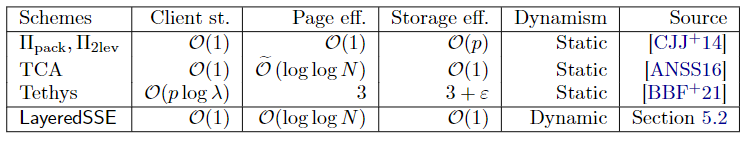
\includegraphics[scale=0.5]{table1.png}
  \caption{高效页面SSE方案。N表示数据库的总大小,p是每页元素的数量,$\varepsilon$ > 0是一个任意小的常数,$\lambda$ 是安全参数。页面效率、存储效率和客户端存储在章节3.1.2中定义。}
  \label{table1} %这样,就可以通过~\ref{fig_1}引用图片了
\end{figure}

\begin{figure}[ht]
  \centering
  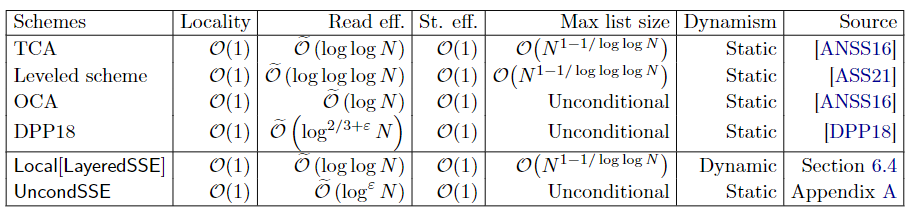
\includegraphics[scale=0.4]{table2.png}
  \caption{具有定域性和存储效率的SSE方案。N表示数据库的总大小,$\varepsilon$ > 0是一个任意小的常数。局部性、读效率和存储效率的定义见章节3.1.2。}
  \label{table2} %这样,就可以通过~\ref{fig_1}引用图片了
\end{figure}

\begin{itemize}
  \item \textbf{动态高效页面SSE。}我们首先构建一个动态页面高效SSE方案LayeredSSE。LayeredSSE实现存储效率O(1),页面效率O(log log N)。与之前关于内存高效SSE的工作一致,LayeredSSE的技术核心是一种新的动态分配方案L2C。L2C是所谓的“2-choice”算法的加权变体,在资源分配文献中臭名昭著。(更多细节在技术概述中提供。)因此,L2C具有独立的利益。
  \item \textbf{泛型局部变换。}我们将介绍泛型局部变换。在输入任何具有特定特征的页效率方案PE-SSE时,称为页长隐藏SSE,通用局部变换输出一个局部SSE方案Local[PE-SSE]。粗略地说,如果PE-SSE有客户端存储O(1),存储效率O(1),页面效率O(P),那么Local[PE-SSE]的存储效率O(1),读取效率O(P)。关于局部性,关键特征是如果PE-SSE在查询最多一个页面大小的列表时具有局部性O(L),那么Local[PE-SSE]在查询任何大小的列表时具有局部性O(L + log log N)。因此,局部构造可以看作是将具有弱局部性的方案引导到具有强得多的局部性的方案。
  
  泛型局部转换还强调了页面效率和局部性目标之间的有趣联系。最初,局部性和页面效率作为不同的性能标准被引入,分别针对两种最广泛的存储介质:硬盘驱动器和固态驱动器。在\cite{AngleBossuat2021SSEAS}中已经观察到,具有局部L和读效率R的方案必须具有最多R + 2L的页效率。从这个意义上说,页面效率是一个“更容易”的目标。令人惊讶的是,使用泛型局部变换,我们在相反的方向上构建了一个连接:我们使用高效页面方案作为构建块来获得局部方案。理论上讲,这显示了两个目标之间的强烈联系。在实际层面上,它提供了同时实现这两个目标的策略。
  \item \textbf{动态本地SSE。}通过将通用局部变换应用于LayeredSSE页效率方案,我们立即获得了一个动态SSE方案Local[LayeredSSE],其存储效率O(1),局域性O(1),读取效率O(log log N)。构造是有条件的:它要求最长列表的大小为$\mathcal{O}\left(N^{1-1 / \log \log N}\right)$。Local[LayeredSSE]的渐近性能与[ANSS16]的第二个静态结构完全匹配,包括最大列表大小的条件:动态不需要额外的代价。特别是,Local[LayeredSSE]匹配[ASS21]中SSE方案的下界,使用[ASS21]称为“分配方案”构建,这表明即使在动态设置中也可以匹配边界。
  \item \textbf{静态设置中无条件的本地SSE。}来自[ANSS16]的原始1-choice方案无条件地实现O(1)存储效率,O(1)局部性和O(log N)读取效率。在[DPP18]中,对于任意常数ε > 0,读取效率提高到$\mathcal{O}\left(\log ^{2 / 3+\varepsilon} N\right)$。这是迄今为止唯一一个无条件实现亚对数效率的SSE建设。通过将泛型局部变换应用于Tethys的变体[BBF+21],并结合[DPP18]启发的技术,我们获得了一个无条件静态SSE方案,对于任何常数ε > 0,它具有存储效率O(1),局域性O(1)和读取效率$\mathcal{O}\left(\log ^{\varepsilon} N\right)$。据我们所知,这是最接近Cash和Tessaro的不可能结果的结构,它表明O(1)局部性、存储效率和读取效率同时是不可能的。
\end{itemize}

\textbf{关于向前安全的说明。}在这项工作中构建的SSE方案在搜索过程中有一个标准的“最小”泄漏剖面:即搜索泄漏搜索模式和访问模式。对于我们的动态方案,更新操作会泄漏正在更新的列表的标识符,在某些情况下还会泄漏列表的长度。因此,我们的动态方案不是前向安全的。潜在的问题是前向安全性和内存效率的目标似乎从根本上是不一致的。事实上,局部性要求与相同关键字相关联的标识符必须彼此靠近地存储;向前-隐私要求插入新标识符的位置应该独立于与其关联的关键字。这个问题已经在[Bos16]中提到了,他声称“对于动态方案,局部性和前向隐私是两个不可调和的概念”。我们建议读者参考[Bos16]以获得关于该问题的更多讨论。我们把对这个问题的进一步分析留给以后的工作。
\section{技术概述}
这项工作包含几个结果,由泛型局部转换连接在一起。因此,我们认为将它们放在一篇论文中是有益的。这就需要引入一些不同的分配机制。我们努力在本节中对这些机制作一个清楚的概述。形式化的规范、定理和证明将在后续章节中介绍。

首先回顾一些经过充分研究的分配机制是有帮助的。在接下来的内容中,“具有压倒性的概率”等同于“除了可忽略不计的概率”(在通常的密码学意义上),而“具有高概率”仅仅意味着在某种意义上概率接近1,但不一定是压倒性的。

一个选择分配。在单选分配中,n个球被扔进n个箱子。每个球被插入一个独立且均匀随机选择的箱子(通过哈希球的标识符)。使用切尔诺夫边界的标准分析表明,在插入过程的结果中,加载最多的bin包含O(log n)个球,具有高概率[JK77]。(对于任意f = ω(1),绝大多数概率最多有O(f (n) log n)个球。)

两个网络分配。同样,n个球被扔进n个箱子。对于每个球,两个箱子被独立且均匀地随机选择(例如通过哈希一个球的标识符)。在插入球的时候,球被插入两个箱子中含有最少的球。Azar等人的一个著名结果表明,在插入过程的结果中,加载最多的bin包含O(log log n)个球,概率很高[ABKU94]。(后来证明该结果以压倒性的概率成立[RMS01]。)

布谷鸟散列。布谷鸟哈希是由Pagh和Rodler [PR04]引入的一种经典哈希方案。它在密码学中有许多应用:其中,无关算法(cf. [CGLS17],以及其中的引用),私有集交集[PSSZ15],以及最近的可搜索加密[PPYY19,BBF+21]。在布谷鸟哈希中,n个球被插入到(2 + ε)n个单元中,其中ε > 0是一个任意小的常数。每个格子最多可以容纳一个球。对于每个球,两个单元格被独立且均匀地随机选择(例如通过哈希球的标识符)。球被插入两个细胞中的一个。如果该单元已经被占用,则占用的球被移动到其他可能的目标单元,可能会产生连锁反应。Pagh和Rodler已经证明了插入在预期do (log n)时间内终止[PR04](包括在插入失败的情况下,用一个新的哈希函数重建整个表的平摊代价)。最后,类似于二选一分配,每个球被存储在两个可能的位置之一。由于更复杂的插入算法(允许移动已经放置的球),负载最多的单元格(根据定义)的负载为1,而不是O(log log n)的两种选择分配。为了实现可以忽略不计的失败概率,加密应用程序通常使用带有隐藏的布谷鸟哈希[KMW10]。
\subsection{分层的两种选择分配}
我们的第一个目标是构建一个动态页面高效方案。让我们从静态情况开始,总结一下这需要什么。正如在介绍中所解释的,要实现单关键字SSE,我们希望在不受信任的服务器上存储任意大小的列表。可以使用对称加密以一种简单的方式来隐藏列表的内容。主要的挑战是如何将列表存储在服务器内存中,以这样一种方式访问一个列表不会显示关于其他列表长度的信息。

在页面效率方案的情况下,这个挑战可以总结如下。我们有一组列表,总共包含N个项目。我们还得到了一个页面大小p,它表示一个物理内存页面中可以容纳的项的数量。服务器的内存被视为一个页面数组。我们希望将列表存储在服务器内存中,考虑到三个目标。

\begin{enumerate}
  \item 为了存储所有列表,我们总共使用S⌈N/p⌉页的服务器内存,其中S称为分配方案的存储效率。我们想让S尽可能小。
  \item 任何长度为ℓ的列表都可以通过访问服务器内存中最多P个⌈ℓ/ P个⌉的页面来检索,其中P称为分配方案的页面效率。我们希望P尽可能小。
  \item 最后,服务器为检索给定列表而访问的页面不应该依赖于其他列表的长度。
\end{enumerate}

前两个目标正是箱子装箱算法的目标。第三个目标是安全目标:它规定服务器执行的内存访问模式不应该泄露某些信息。因此,目标涉及到无关的或数据独立的算法。在[BBF+21]中,实现这三个目标的框架被形式化为数据独立包装(DIP)。

为了便于表示,我们将关注所有列表的大小最多为一页的情况。如果一个列表的长度超过一页,一般的想法是它将被分割成一页的块,加上最后一个最多一页的块;然后,每个块将被分配方案视为一个单独的列表。我们假设从现在开始列表的长度小于一页。

简而言之,[BBF+21]提出的实例化DIP方案的想法是使用杜鹃哈希的加权变体。更详细地说,对于每个列表,通过散列列表的标识符,统一随机地选择两个页面。然后,列表的每个元素将存储在两个指定页面中的一个页面中,或一个stash中。隐藏存储在客户端。为了选择每个列表如何在其三个可能的目的地(两个选择的页面,或存储)之间分割,[BBF+21]使用了最大流量算法。这个算法的细节与我们的目的无关。重要的一点是,在检索列表时,服务器访问两个统一随机的页面。显然,这不会向服务器透露关于其他列表长度的信息。由此产生的算法,称为Tethys,实现了存储效率O(1),页面效率yo(1),客户端存储ω(log λ)页(用于存储隐藏)。

在本文中,我们希望建立一个动态SSE。为此,底层分配方案需要允许新的更新操作。更新操作允许客户端向列表中添加一个新项,将其长度增加1。安全性目标本质上与静态情况相同:算法为了更新给定列表而访问的页面不应该依赖于其他列表的长度。

Tethys不适合作为动态方案的基础,因为它不支持有效的与数据无关的更新过程:在更新期间向单元格插入元素时,更新过程需要访问其他单元格,其访问模式本质上是与数据相关的。相反,一个自然的想法是使用两种选择分配方案的加权变体。使用两种选择分配,更新期间的访问模式很简单:只需要读取与正在更新的列表关联的两个目标桶。然后将新项插入到当前包含较少项的两个桶中。

实例化该方法将需要一个二选一分配的加权变体,如下所示:给定一个多集列表大小{ℓi: 1≤i≤k},ℓi≤p和∑ℓi = N,在二选一分配过程的结果为O(N/p)个桶时,加载最多的桶以压倒性的概率包含O(p log log N)个项目。然而,这种形式的结果似乎是一个长期存在的开放问题(一些相关的部分结果在[BFHM08]中讨论)。文献[TW07, TW14]中已经研究了加权项目的二选一过程,但据我们所知,所有现有的结果都假设球的重量取样相同且独立于足够平滑的分布。即使不考虑分布上的约束,在我们的设置中,我们甚至不能假设列表长度是独立绘制的:在SSE安全模型中,列表是由对手任意选择和更新的。

为了我们的目的,我们需要一个无分布的陈述:我们只知道每个列表大小的边界p,以及所有列表总大小的边界N。我们想要一个O(p log log N)加载最多的桶大小的上限,它适用于满足这些约束的任何一组列表大小。这种形式的结果是已知的一种选择分配过程[BFHM08](具有O(p log N)上限),但同一篇文章表明,相同的技术不能扩展到两种选择过程。

为了解决这一问题,我们引入了一种分层加权二选择分配算法L2C。L2C具有与(加权)二选算法相同的基本行为:对于每个球,均匀随机地选择两个箱子作为可能的目的地。唯一的区别是如何在两个目标箱子中选择实际插入球的箱子。最自然的选择是将球存储在当前负载最小的容器中,其中容器的负载是当前所包含的球的重量之和。相反,我们使用一个稍微复杂一点的决策过程。简而言之,我们将球的可能权重划分为O(log log λ)子区间,并对每个子区间内的球独立执行决策过程。对于第一个子区间(保留最小的权重),我们使用加权的单选过程,而对于其他子区间,我们使用未加权的二选过程。

这种结构的要点在于,它的分析可以简化为加权的一项选择过程和非加权的两项选择过程的分析,这两项选择过程以强大的分析技术而闻名。我们利用这些技术来证明L2C在负载最多的bin的负载上实现了所需的无分布保证。在实践中,这意味着我们有一个分配算法,在大多数意图和目的下,表现得像二选一分配的加权变体,并且可以相对轻松地获得无分配保证。多项选择分配过程在计算机科学的某些领域普遍存在,这使得它成为独立利益的结果。

LayeredSSE方案是通过在L2C之上增加一层加密和密钥管理,使用SSE文献中的标准技术来获得的,尽管需要注意更新。详情请参阅第5.2节。


\subsection{泛型局部变换}
在Crypto 2018上,Asharov等人确定了构建本地SSE的两个主要范例[ASS18]。第一个是分配范式,它通常使用多项选择分配方案的变体,或布谷鸟哈希法。第二种是“垫-拆”方法。高效内存SSE的主要困难在于将不同大小的列表打包在一起。填充和分割方法的思想是根据列表的大小分别存储列表,从而避免了这个问题。实现这一点最简单的方法是填充所有列表的长度到下一个2的幂。这将产生log N个列表长度的可能值。所有给定长度的列表都可以存储在一起,例如,使用标准哈希表。由于我们不想透露每种长度的列表的数量,因此每一层的哈希表都需要进行维数划分,以便能够接收整个数据库。因此,基本的“垫-拆”方案的存储效率为O(log N),但很容易实现O(1)局部性和读取效率。

对于泛型局部变换,我们引入了溢出SSE (OSSE)的概念。OSSE在所有方面都像SSE方案,除了在其设置和更新期间,它可能拒绝存储一些列表元素。这样的元素称为溢出。OSSE打算用作overaching SSE构造中的子组件。OSSE方案用于存储部分数据库,而溢出元素则使用单独的机制存储。OSSE的概念之前并没有形式化,但事后看来,OSSE的使用可能被视为隐含在几个现有的结构中[DPP18, ASS18, BBF+21]。为了便于阐述,我们选择在这里显式地介绍它。

现在我们来解释泛型局部变换。填充和分割方法的主要限制是它在存储中创建了log N的开销。因此,泛型局部变换的高级思想是使用OSSE存储数据库中除1/ log N以外的所有数据。然后使用“填充-拆分”变体存储N/ log N个溢出元素。这样做的目的是受益于填充和分割方法的高效率,而不必支付log N的存储开销

然而,这种方法有一个微妙但重要的问题。给定的列表可以完全存储在OSSE方案中,或者只存储部分,或者根本不存储。在我们稍后将使用的OSSE方案(以及之前工作中隐含的OSSE)中,服务器应该无法区分这三种情况,否则安全性就会崩溃。为了解决这个问题,我们采取如下措施。

让我们假设所有的列表都被填充到下一个2的幂。对于构造的填充和分割部分,我们创建了log N个SSE实例,每个实例对应一个可能的列表大小。我们将每个实例称为一个层。如果一个列表的大小为ℓ,它的溢出元素将存储在处理大小为ℓ的列表的层中,而不管有多少元素从该列表的OSSE溢出。

OSSE提供的关于溢出元素的唯一保证是它们的总数不= O(N/ log N)。因此,如果我们关注处理大小为ℓ的列表的层,该层将接收最多的元素。这些元素将被分割成大小不超过ℓ的列表(对应于溢出元素的集合,对于原始数据库中大小为ℓ的每个列表)。为了实现整体存储效率O(S),我们希望该层使用O(Sn)存储来存储这些列表。为了实现读效率R,该层还应该能够通过访问最多Rℓ内存位置来检索给定的列表。这就是所有事情都集中在一起的地方:满足这些条件的SSE方案正是页面大小为ℓ、存储效率为S、页面效率为R的高效页面SSE方案。

每一层使用的页面高效方案还需要满足一些额外的属性:首先,当搜索最多一页的列表时,列表的长度不应该泄露。我们称之为propertype -length-hiding。(我们避免使用长度隐藏这个术语,以避免与完全隐藏长度的体积隐藏SSE混淆。)所有现有的高效页结构都具有该属性。其次,我们要求页面高效方案拥有O(1)个客户端存储。本文中的所有结构都满足这个性质,但[BBF+21]中的结构不满足。最后,我们要求该方案在获取单个页面时具有局部性O(1)。所有现有的高效页结构都具有此属性。(最后两个属性可以放宽,但要付出更复杂的公式和语句的代价。)我们称满足这三个性质的SSE方案为合适的。

将所有内容放在一起,通用局部转换将一个合适的页效率方案作为输入,存储效率S和页效率P。它输出一个存储效率S + S ',读取效率P + R '和局部性L '的局部方案,其中S ', R '和L '是底层OSSE的存储效率,读取效率和局部性。接下来还需要解释如何构建具有O(N/ log N)个溢出项的本地OSSE方案。

\subsection{ClipOSSE: O(N/ log N)个溢出项的OSSE方案}
在2016年STOC上,Asharov等人引入了所谓的“二维”版本的一项选择和两项选择分配,目的是建立本地SSE。单选变体的工作原理如下。考虑一个有N个元素的SSE数据库。分配m = O (N/ log N)个桶,初始为空。对于数据库中每个长度为ℓ的列表,随机统一选择一个桶。列表的第一个元素被插入到该bucket中。列表的第二个元素被插入到下一个bucket中(假设bucket的顺序是固定的,当到达最后一个bucket时,顺序会改变),第三个元素被插入到之后的bucket中,依此类推,直到所有列表元素都被插入。因此,假设ℓ≤m,所有列表元素都被放置在ℓ连续的桶中,每个桶中有一个元素。一个非常类似于对一项选择过程的通常分析的分析表明,在压倒性的概率下,加载最多的桶接收最多τ =′O (log N)个元素。为了从这个分配方案构建一个静态SSE方案,每个桶都被填充到最大大小τ并加密。搜索查询以自然的方式进行。

这样的方案产生存储效率O(1)、位置O(1)(因为检索列表相当于读取连续的桶)和读取效率O(log N)(因为检索长度为ℓ的列表需要读取ℓ个桶,每个桶的大小τ = O(log N))。为了构建ClipOSSE,我们从相同的前提开始,但是在阈值τ =′O (log log N)处“截取”桶。也就是说,每个bucket最多只能接收τ元素。无法匹配的元素被溢出。

在标准的一项选择过程中,将n个球i.i.d.扔到n个箱子中,不难证明在高度τ = O(log log n)处剪切箱子会以压倒性的概率导致最多O(n/ log n)个溢出元素。事实上,通过在τ的选择中调整乘法常数,对于任何给定的常数d,溢出元素的数量可以变成O(n/ logd n)。我们表明,这种形式的结果仍然适用于前面概述的二维一选过程(一种近似的变体)。结果是有条件的:它要求最大列表大小为O(N/polylog N)。(这种形式的条件是必要的,因为当最大列表大小接近N/ log N时,结果会失败。)相应定理的证明是这项工作中最具技术挑战性的部分,它依赖于凸性论证和随机支配性论证的结合。在D中给出了证明的概述,所以我们省略了更多的讨论。

最后,在最大列表大小为O(N/polylog N)的条件下,ClipOSSE实现了存储效率O(1),局域性O(1)和读取效率O(log log N),有O(N/ logd N)个溢出元素(对于我们选择的任何固定常数d)。本文中通用局部转换的所有应用程序都使用ecliposse作为底层OSSE。(这就是为什么我们为应用于页效率方案PE-SSE的通用局部转换编写Local[PE-SSE],而不将底层OSSE作为显式参数。)

\subsection{开销为O(log log N)的动态本地SSE}
通过使用ClipOSSE作为底层OSSE, LayeredSSE作为页面高效方案的泛型局部变换,我们得到了Local[LayeredSSE]。Local[LayeredSSE]方案的存储效率为O(1),局域性为O(1),读取效率为O(log log N)。这个结果来自于关于泛型局部变换的主要定理,不需要任何新的分析。

Local[LayeredSSE]是一个条件方案:它要求最长列表的长度为O(N 1−1/ log log λ)。原因很微妙。ClipOSSE本身有一个条件,即最长的列表是O(N/polylog N),这个条件要求较低。这种情况的原因归结为LayeredSSE只有在方案中的页面数至少为Ω(λ1/ log log λ)的情况下才能实现可以忽略不计的失败概率。更普遍的是,在一般的两种选择分配过程中,即使是标准的、未加权的过程,箱子的数量也是如此。条件是最优的:[ASS21]表明任何亚对数“基于分配”的方案都必须是有条件的,并给出了条件的一个边界。Local[PE-SSE]匹配该边界。

\section{方法}
范例
\subsection{方法1}
范例
\subsection{方法2}
范例
\section{实验}
范例
\section{结论}
范例

\bibliographystyle{unsrt}
\bibliography{ref}

\end{document}

